\documentclass[8pt]{article}
\usepackage{amssymb}
\usepackage{hyperref}
\usepackage{pgfplots}
\usepackage{placeins}
\usepackage{array}
\usepackage{tikz}
\usepackage{circuitikz}
\usetikzlibrary{circuits.logic.US, circuits.ee.IEC, positioning}
\usepackage{amsmath}
\usepackage{graphicx}
\usepackage[T1]{fontenc}
\usepackage[utf8]{inputenc}
\usepackage{listings}
\usepackage{xcolor}
\usepackage{geometry}
\geometry{margin=0.2in}

\lstdefinelanguage{SystemVerilog}{
  morekeywords={module, endmodule, logic, bit, int, enum, struct,
    always_ff, always_comb, initial, final, interface, modport, property,
    assert, class, rand, constraint, generate, endgenerate, if, else, begin, end},
  sensitive=true,
  morecomment=[l]{//},
  morecomment=[s]{/*}{*/},
  morestring=[b]",
}

\lstset{
  language=SystemVerilog,
  basicstyle=\ttfamily\footnotesize,
  keywordstyle=\color{blue}\bfseries,
  commentstyle=\color{gray}\itshape,
  stringstyle=\color{red},
  frame=single,
  breaklines=true,
  postbreak=\mbox{\textcolor{red}{$\hookrightarrow$}\space},
}

\begin{document}

\noindent Username (e.g. ppete9): \makebox[1.5in]{\hrulefill} \\[10pt]


\begin{table}[h]
  \centering
  \begin{tabular}{|l|l|}
    \hline
    \textbf{Rule}           & \textbf{Expression}                                                                            \\ \hline
    Commutativity           & $X + Y = Y + X$                                                                                \\
                            & $X \cdot Y = Y \cdot X$                                                                        \\ \hline
    Associativity           & $(X + Y) + Z = X + (Y + Z)$                                                                    \\
                            & $(X \cdot Y) \cdot Z = X \cdot (Y \cdot Z)$                                                    \\ \hline
    Distributivity          & $X \cdot Y + X \cdot Z = X \cdot (Y + Z)$                                                      \\
                            & $(X + Y) \cdot (X + Z) = X + Y \cdot Z$                                                        \\ \hline
    Covering                & $X + X \cdot Y = X$                                                                            \\
                            & $X \cdot (X + Y) = X$                                                                          \\ \hline
    Combining               & $X \cdot Y + X \cdot Y = X$                                                                    \\
                            & $(X + Y) \cdot (X + Y) = X$                                                                    \\ \hline
    Consensus               & $X \cdot Y + X \cdot Z + Y \cdot Z = X \cdot Y + X' \cdot Z$                                   \\
                            & $(X + Y) \cdot (X + Z) \cdot (Y + Z) = (X + Y) \cdot (X + Z)$                                  \\ \hline
    Generalized Idempotency & $X + X + \dots + X = X$                                                                        \\
                            & $X \cdot X \cdot \dots \cdot X = X$                                                            \\ \hline
    DeMorgan's Theorems     & $(X_1 \cdot X_2 \cdot \dots \cdot X_n)' = X_1' + X_2' + \dots + X_n'$                          \\
                            & $(X_1 + X_2 + \dots + X_n)' = X_1' \cdot X_2' \cdot \dots \cdot X_n'$                          \\ \hline
    Generalized DeMorgan's  & $F(X_1, X_2, \dots, X_n, +, \cdot) = F(X_1, X_2, \dots, X_n, \cdot, +)'$                       \\ \hline
    Shannon's Expansion     & $F(X_1, X_2, \dots, X_n) = X_1 \cdot F(1, X_2, \dots, X_n) + X_1' \cdot F(0, X_2, \dots, X_n)$ \\
                            & $F(X_1, X_2, \dots, X_n) = [X_1 + F(0, X_2, \dots, X_n)] \cdot [X_1' + F(1, X_2, \dots, X_n)]$ \\ \hline
    Dual                    & Interchange $+$ with $\cdot$, and $0$ with $1$                                                 \\ \hline
  \end{tabular}
\end{table}

\begin{lstlisting}[language=SystemVerilog]
//    !  : Logical NOT, ~ : Bitwise NOT
//    && : Logical AND, & : Bitwise AND
//    || : Logical OR,  | : Bitwise OR
//    ^  : Bitwise XOR
//    ~^ : Bitwise XNOR
//    == : Equality,    === : Case Equality (4-state)
//    != : Inequality,  !== : Case Inequality (4-state)
\end{lstlisting}

\begin{lstlisting}
module top_module (
  input  logic x1,
  input  logic y1,
  output logic f1
);
  // Module internals here
endmodule

module sub_module (
  input  logic x2,
  input  logic y2,
  output logic f2
);
  // Submodule internals here
endmodule

sub_module sub_inst(.x2(x1), .y2(y1), .f2(f1));
\end{lstlisting}

\begin{lstlisting}
// Sequential (synchronous) logic
always_ff @(posedge clk or posedge rst) begin
  if (rst)
    out <= 0;
  else
    out <= ~out;
end

// Combinational logic
always_comb begin
  // assignments that depend solely on input combinatorics
end
\end{lstlisting}

\begin{lstlisting}
interface simple_if (input logic clk);
  logic data;
  modport master (output data);
  modport slave  (input  data);
endinterface
\end{lstlisting}

\renewcommand{\arraystretch}{1.5}
\newcommand{\gateBox}[3]{
  \begin{minipage}[t]{0.45\textwidth}
    \centering
    \textbf{#1}\\[5pt]
    #2\\[5pt]
    #3
  \end{minipage}
}

\begin{flushleft}
  \begin{tabular}{>{\centering\arraybackslash}m{0.2\textwidth} >{\centering\arraybackslash}m{0.2\textwidth} >{\centering\arraybackslash}m{0.2\textwidth} >{\centering\arraybackslash}m{0.2\textwidth}}
    \gateBox{Buffer}{%
      \begin{tabular}{|c|c|}
        \hline
        A & Output \\ \hline
        0 & 0      \\ \hline
        1 & 1      \\ \hline
      \end{tabular}
    }{%
      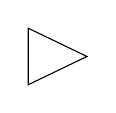
\begin{tikzpicture}[circuit logic US]
        \node [buffer gate, draw, logic gate inputs=1, anchor=output] {};
      \end{tikzpicture}
    }
     &
    \gateBox{NOT}{%
      \begin{tabular}{|c|c|}
        \hline
        A & Output \\ \hline
        0 & 1      \\ \hline
        1 & 0      \\ \hline
      \end{tabular}
    }{%
      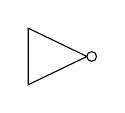
\begin{tikzpicture}[circuit logic US]
        \node [not gate, draw, logic gate inputs=n] {};
      \end{tikzpicture}
    }
     &
    \gateBox{OR}{%
      \begin{tabular}{|c|c|c|}
        \hline
        A & B & Output \\ \hline
        0 & 0 & 0      \\ \hline
        0 & 1 & 1      \\ \hline
        1 & 0 & 1      \\ \hline
        1 & 1 & 1      \\ \hline
      \end{tabular}
    }{%
      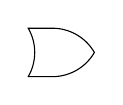
\begin{tikzpicture}[circuit logic US]
        \node [or gate, draw, logic gate inputs=nn] {};
      \end{tikzpicture}
    }
     &
    \gateBox{AND}{%
      \begin{tabular}{|c|c|c|}
        \hline
        A & B & Output \\ \hline
        0 & 0 & 0      \\ \hline
        0 & 1 & 0      \\ \hline
        1 & 0 & 0      \\ \hline
        1 & 1 & 1      \\ \hline
      \end{tabular}
    }{%
      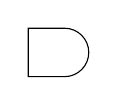
\begin{tikzpicture}[circuit logic US]
        \node [and gate, draw, logic gate inputs=nn] {};
      \end{tikzpicture}
    }
    \\[2em]
    \gateBox{NAND}{%
      \begin{tabular}{|c|c|c|}
        \hline
        A & B & Output \\ \hline
        0 & 0 & 1      \\ \hline
        0 & 1 & 1      \\ \hline
        1 & 0 & 1      \\ \hline
        1 & 1 & 0      \\ \hline
      \end{tabular}
    }{%
      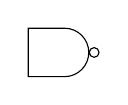
\begin{tikzpicture}[circuit logic US]
        \node [nand gate, draw, logic gate inputs=nn] {};
      \end{tikzpicture}
    }
     &
    \gateBox{NOR}{%
      \begin{tabular}{|c|c|c|}
        \hline
        A & B & Output \\ \hline
        0 & 0 & 1      \\ \hline
        0 & 1 & 0      \\ \hline
        1 & 0 & 0      \\ \hline
        1 & 1 & 0      \\ \hline
      \end{tabular}
    }{%
      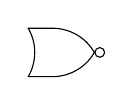
\begin{tikzpicture}[circuit logic US]
        \node [nor gate, draw, logic gate inputs=nn] {};
      \end{tikzpicture}
    }
     &
    \gateBox{XOR}{%
      \begin{tabular}{|c|c|c|}
        \hline
        A & B & Output \\ \hline
        0 & 0 & 0      \\ \hline
        0 & 1 & 1      \\ \hline
        1 & 0 & 1      \\ \hline
        1 & 1 & 0      \\ \hline
      \end{tabular}
    }{%
      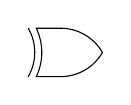
\begin{tikzpicture}[circuit logic US]
        \node [xor gate, draw, logic gate inputs=nn] {};
      \end{tikzpicture}
    }
     &
    \gateBox{XNOR}{%
      \begin{tabular}{|c|c|c|}
        \hline
        A & B & Output \\ \hline
        0 & 0 & 1      \\ \hline
        0 & 1 & 0      \\ \hline
        1 & 0 & 0      \\ \hline
        1 & 1 & 1      \\ \hline
      \end{tabular}
    }{%
      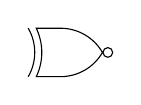
\begin{tikzpicture}[circuit logic US]
        \node [xnor gate, draw, logic gate inputs=nn] {};
      \end{tikzpicture}
    }
  \end{tabular}
\end{flushleft}

\begin{center}
  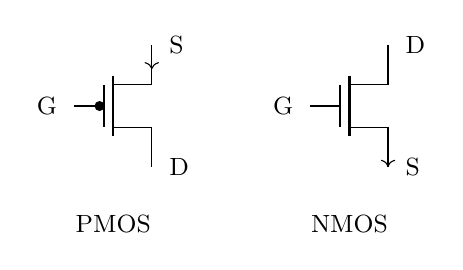
\begin{tikzpicture}[circuit ee IEC, every node/.style={font=\small}]
    % PMOS Transistor
    \draw (0,0) node[pmos, rotate=0] (PMOS) {};
    \node[below=0.5cm of PMOS] {PMOS};

    % PMOS Labels
    \node[left=0.1cm of PMOS.gate] {G};
    \node[right=0.1cm of PMOS.drain] {D};
    \node[right=0.1cm of PMOS.source] {S};

    % PMOS Arrows
    \draw[->] (PMOS.source) -- ++(0, -0.3);

    % NMOS Transistor
    \draw (3,0) node[nmos, rotate=0] (NMOS) {};
    \node[below=0.5cm of NMOS] {NMOS};

    % NMOS Labels
    \node[left=0.1cm of NMOS.gate] {G};
    \node[right=0.1cm of NMOS.drain] {D};
    \node[right=0.1cm of NMOS.source] {S};

    % NMOS Arrows
    \draw[<-] (NMOS.source) -- ++(0, 0.3);
  \end{tikzpicture}
\end{center}

\begin{table}[h]
  \centering
  \begin{tabular}{|l|l|l|}
    \hline
    \textbf{Parameter} & \textbf{PMOS} & \textbf{NMOS} \\
    \hline
    Substrate Type     & n-type        & p-type        \\
    Threshold Voltage  & Negative      & Positive      \\
    \hline
  \end{tabular}
\end{table}

\[
  \begin{array}{|c|c|c|}
    \hline
    \text{Gate}            & \text{PMOS Configuration} & \text{NMOS Configuration} \\
    \hline
    \text{OR} (A + B)      & \text{Parallel}           & \text{Series}             \\
    \text{AND} (A \cdot B) & \text{Series}             & \text{Parallel}           \\
    \hline
  \end{array}
\]


% Noise margins

% Transition time

\begin{itemize}
  \item[$t_{pHL}$:] The time between an input change and the corresponding output change
        when the output changes from HIGH to LOW.
  \item[$t_{pLH}$:] The time between an input change and the corresponding output change
        when the output changes from LOW to HIGH.
  \item Note: $t_p$ is measured from the 50\% crossing
        of the input to the 50\% crossing of the output
\end{itemize}

% Power consumption of CMOS

\[  P = cV^2 f \]
\end{document}